\section{完整敏感性数据}
\label{chapter:S2}

% block-id: S2.geometry.heading
\hypertarget{S2.geometry.heading}{}
\subsection{几何采样与离散换位}

% block-id: S2.geometry.p1
\hypertarget{S2.geometry.p1}{}
图~\ref{fig:geometry_comparison} 展示直束、单级、传统多级与跨层中心线。几何记录包括股线身份、周期、间隙、曲率、实际弧长和铜体积，400、800、1600 轴向采样及 60 项检查支持这些量的采样一致性。所示 24 股、0.100 mm 铜径结构的名义铜面积约为 0.1885 mm²，用于说明几何构造；满足至少 5 mm² 铜面积的结构需另行建立并验证。三维视角用于观察空间路径，电磁性能由相应场路模型评价。

% block-id: S2.figure.geometry_comparison
\hypertarget{S2.figure.geometry_comparison}{}
\begin{figure*}[!htbp]
\centering
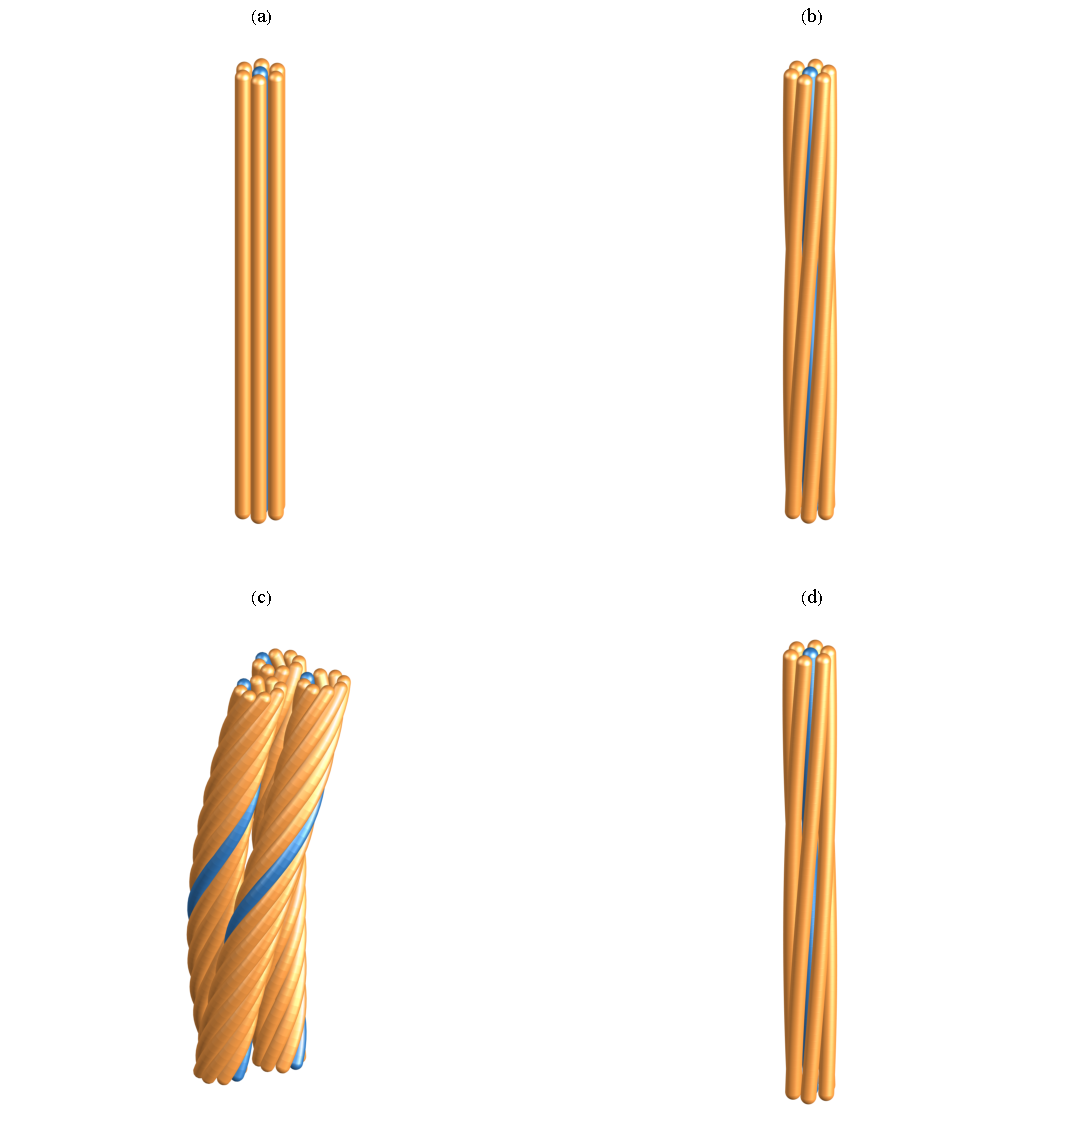
\includegraphics[width=\linewidth,height=.72\textheight,keepaspectratio]{../../assets/zh-CN/geometry_comparison.pdf}
\caption{股线中心线的三维结构比较。 面板依次展示直束、单级、传统多级局部和跨层结构。}
\label{fig:geometry_comparison}
\end{figure*}

% block-id: S2.geometry.p2
\hypertarget{S2.geometry.p2}{}
当前 DTM/iDTM 演示采用 \eqref{eq:E06} 的加性离散块。对于同一组带权阻抗块，求和结果对排列顺序保持不变，因此该实现可验证身份映射和给定块的电路叠加。真实换位路径的比较还需考虑位置随长度的变化、层级间的非交换关系、局部场及端接条件。与文献 \cite{P01,N01} 对照时，这些具体假设决定两种实现具有多大可比性。

% block-id: S2.rt0.heading
\hypertarget{S2.rt0.heading}{}
\subsection{RT0 长方体外场算例}

% block-id: S2.rt0.p1
\hypertarget{S2.rt0.p1}{}
算例为 1×1×2 mm 均质铜长方体，频率 200 kHz，外加 Bz=1 mT RMS，净输运电流为零。三分量电流以面通量自由度表示，分别检查连续性、端口约束和外场功率。采用 q=14 积分时，8192、16000、27648 单元的损耗为 0.927463、0.933539、0.936927 mW；连续两次细化变化为 0.655090\% 和 0.362916\%，低于 1\% 目标。末档提高至 q=18 后，损耗与复面通量的相对变化分别为 1.55×10⁻⁸ 和 1.39×10⁻⁸，低于 0.1\% 积分目标，见 图~\ref{fig:rt0_spatial}。

% block-id: S2.figure.rt0_spatial
\hypertarget{S2.figure.rt0_spatial}{}
\begin{figure}[!htbp]
\centering
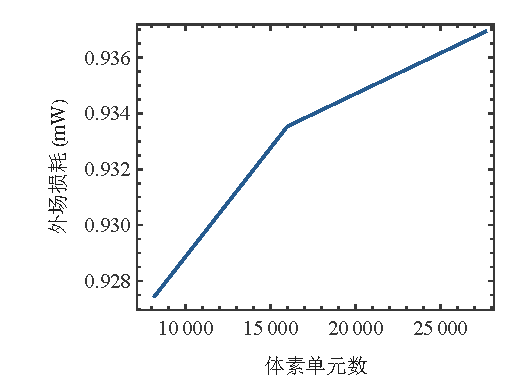
\includegraphics[width=\linewidth,height=.72\textheight,keepaspectratio]{../../assets/zh-CN/rt0_spatial.pdf}
\caption{RT0 空间与积分对照。 铜长方体为 1×1×2 mm，200 kHz、1 mT RMS 外场、零净输运。 q14 空间序列与末档 q18 对照使用相同外场工况。}
\label{fig:rt0_spatial}
\end{figure}

% block-id: S2.rt0.p2
\hypertarget{S2.rt0.p2}{}
切面和矢量图分别见 图~\ref{fig:rt0_sections}、图~\ref{fig:rt0_vectors}，均由保存的面通量恢复。单元中心电流由相对两面的通量平均后除以面面积得到；单元平均损耗密度采用完整 RT0 局部重叠积分，因此包含单元内电流变化。箭头表示零相位时刻电流的实部，并采用统一长度比例，色标表示复 RMS 范数。切面位置和矢量抽样对应图中标注，体积分则使用全部单元。

% block-id: S2.figure.rt0_sections
\hypertarget{S2.figure.rt0_sections}{}
\begin{figure*}[!htbp]
\centering
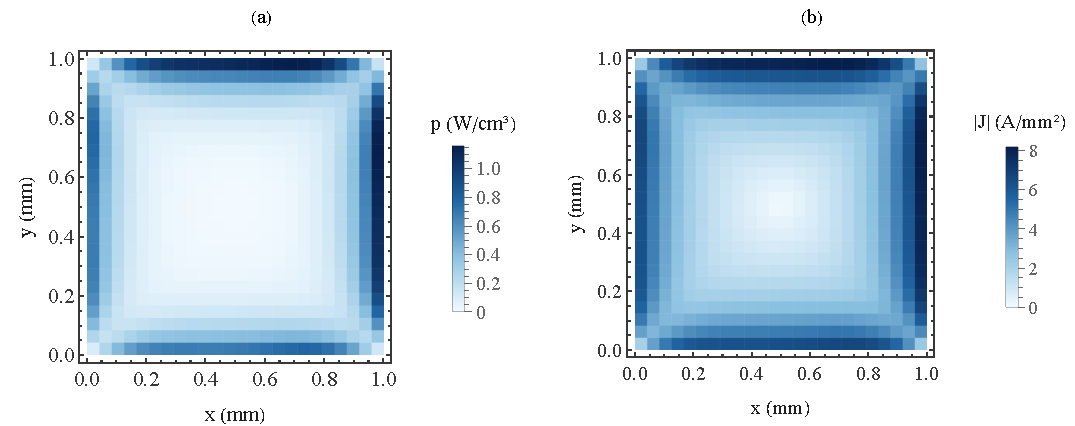
\includegraphics[width=\linewidth,height=.72\textheight,keepaspectratio]{../../assets/zh-CN/rt0_sections.pdf}
\caption{RT0 外场电流与损耗切面。 铜长方体为 1×1×2 mm，200 kHz、1 mT RMS 外场、零净输运。 (a) 单元平均损耗密度；(b) 复 RMS 电流范数。}
\label{fig:rt0_sections}
\end{figure*}

% block-id: S2.figure.rt0_vectors
\hypertarget{S2.figure.rt0_vectors}{}
\begin{figure}[!htbp]
\centering
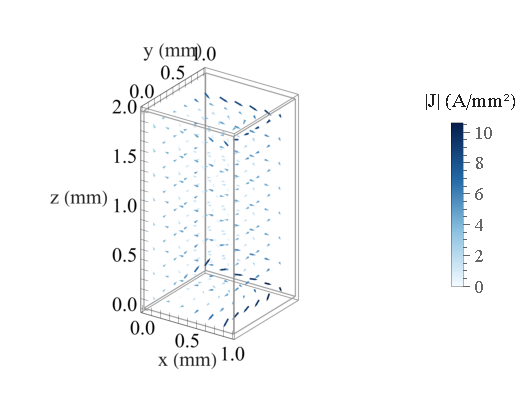
\includegraphics[width=\linewidth,height=.72\textheight,keepaspectratio]{../../assets/zh-CN/rt0_vectors.pdf}
\caption{RT0 重构电流三维矢量。 铜长方体为 1×1×2 mm，200 kHz、1 mT RMS 外场、零净输运。 箭头为固定相位的实部，色标为复 RMS 范数。}
\label{fig:rt0_vectors}
\end{figure}

% block-id: S2.rt0.p3
\hypertarget{S2.rt0.p3}{}
各档记录的 GMRES 迭代次数为 35，真残差满足 10⁻¹¹ 目标。空间与积分比较共同支持固定外场长方体的数值结论，适用范围尚未扩展至曲线 Litz 掩膜、独立边界通量验证和实际输运端接。q=18 原摘要中的缺失指标与失败状态、基于 CSV 的后处理验收，以及致密和矩阵自由实现的资源记录分别列入来源资料，以保持求解和数据解释的对应关系。

% block-id: S2.aphi.heading
\hypertarget{S2.aphi.heading}{}
\subsection{A–φ 圆柱校准与场势诊断}

% block-id: S2.aphi.p1
\hypertarget{S2.aphi.p1}{}
A–φ 模型按 \eqref{eq:E07}，由保存的 A 和 φ 的实际梯度恢复电流。圆柱三档网格分别含 1683、3672、9108 节点，结果见 图~\ref{fig:aphi_gates}。最细档径向 J 校准达到目标，φ 与规范残差在三档中仍未通过，较粗两档 J 也未达到目标。制造解检查支持所检验方程与实现的对应关系，物理圆柱校准则揭示了仍需研究的场势一致性问题。

% block-id: S2.equation.E07
\hypertarget{S2.equation.E07}{}
\hypertarget{E07}{}\begin{equation}\mathbf J=-\sigma\left(j\omega\mathbf A+\nabla\phi\right)\tag{9}\label{eq:E07}\end{equation}

% block-id: S2.figure.aphi_gates
\hypertarget{S2.figure.aphi_gates}{}
\begin{figure}[!htbp]
\centering
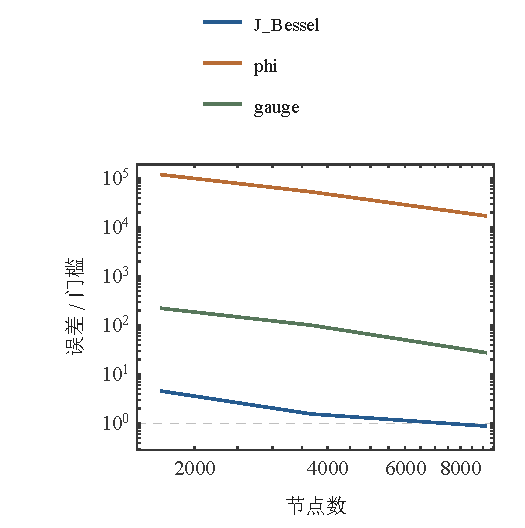
\includegraphics[width=\linewidth,height=.72\textheight,keepaspectratio]{../../assets/zh-CN/aphi_gates.pdf}
\caption{A–φ 圆柱校准指标。 三档网格与各指标门槛分别展示。}
\label{fig:aphi_gates}
\end{figure}

% block-id: S2.aphi.p2
\hypertarget{S2.aphi.p2}{}
图~\ref{fig:aphi_preserved} 使用 128 个具有明确身份的节点样本，分别显示 A、φ、J 和实际 φ 梯度，表示这些采样位置的数值。边界、缩放、导数与后处理的诊断记录，以及直接分解、OOC 和迭代路线的失败原因，共同保留在复现资料中。它们用于进一步区分实现问题与离散误差；当前圆柱结果的物理验收状态为未通过。

% block-id: S2.figure.aphi_preserved
\hypertarget{S2.figure.aphi_preserved}{}
\begin{figure*}[!htbp]
\centering
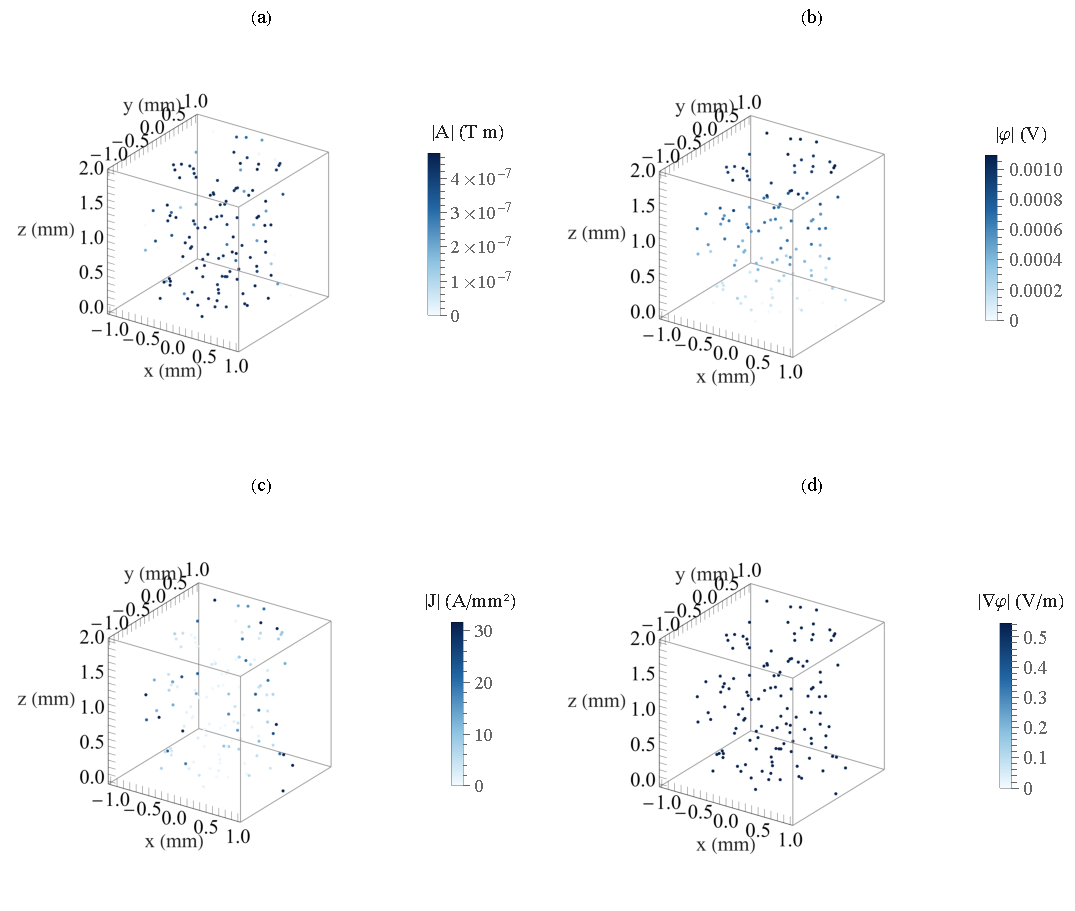
\includegraphics[width=\linewidth,height=.72\textheight,keepaspectratio]{../../assets/zh-CN/aphi_preserved.pdf}
\caption{A–φ 保存场样本。 面板分别给出 A、φ、J 和实际 φ 梯度。}
\label{fig:aphi_preserved}
\end{figure*}

% block-id: S2.ansys.heading
\hypertarget{S2.ansys.heading}{}
\subsection{Ansys 端口验证与能力范围}

% block-id: S2.ansys.p1
\hypertarget{S2.ansys.p1}{}
七股二维端口短测采用 704 单元，包含两个电压基解和第三次实际 ±20 A 场解。公共端电压、逐股复电流与独立功率为这一网格提供场路一致性检查，电流结果见 图~\ref{fig:ansys_seven_current}。其验证范围为单档网格；后续固定网格与精度尝试尚未形成完整三档验收，原生三维 J 表达式探针也未取得可接受的物理解。

% block-id: S2.figure.ansys_seven_current
\hypertarget{S2.figure.ansys_seven_current}{}
\begin{figure}[!htbp]
\centering
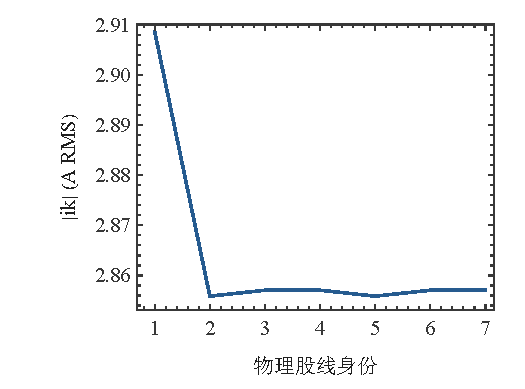
\includegraphics[width=\linewidth,height=.72\textheight,keepaspectratio]{../../assets/zh-CN/ansys_seven_current.pdf}
\caption{Ansys 七股二维复电流。 704 单元有效端口短测给出逐股幅值与相位。}
\label{fig:ansys_seven_current}
\end{figure}

% block-id: S2.ansys.p2
\hypertarget{S2.ansys.p2}{}
图~\ref{fig:ansys_limits} 汇总已核查的 Ansys Student v252 能力：二维最多 2000 个三角形，三维最多 64000 个体单元和 8000 个面单元，计算最多使用 4 核。接口、许可规模和数值精度分别限制可执行的验证。实际端接、曲线 STL 与足铜大束研究需要与目标几何相匹配的许可和网格能力，并完成相应敏感性与功率检查。

% block-id: S2.figure.ansys_limits
\hypertarget{S2.figure.ansys_limits}{}
\begin{figure}[!htbp]
\centering
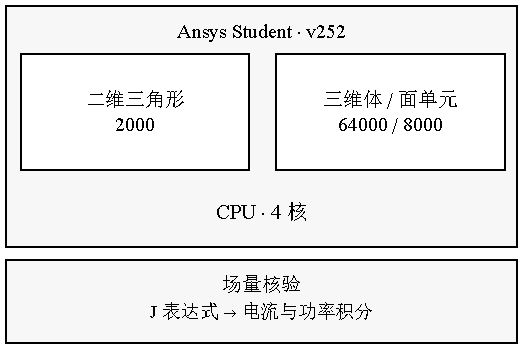
\includegraphics[width=\linewidth,height=.72\textheight,keepaspectratio]{../../assets/zh-CN/ansys_limits.pdf}
\caption{Ansys Student 能力与接口诊断。 Ansys Student v252 的许可规模及场量检查入口。二维上限为 2000 个三角形，三维上限为 64000 个体单元与 8000 个面单元，计算使用至多四核。许可边界来自 rc.1 保存记录，图件来源核对日期为 2026-10-15。}
\label{fig:ansys_limits}
\end{figure}

% block-id: S2.tables
\hypertarget{S2.tables}{}
\begin{table*}[!htbp]
\centering
\caption{单圆线二维校准}
\label{tab:S2.tables-0}
\begingroup\footnotesize
\begin{tabularx}{\textwidth}{>{\raggedright\arraybackslash}X>{\raggedright\arraybackslash}X>{\raggedright\arraybackslash}X>{\raggedright\arraybackslash}X}
\toprule
节点数 & h/a & Rac (mΩ/m) & 电阻相对误差\\
\midrule
353 & 0.24 & 20.1572 & 0.00704525\\
1389 & 0.12 & 20.0208 & 0.000230269\\
5573 & 0.06 & 20.0162 & 1.79233e-06\\
\bottomrule
\end{tabularx}
\endgroup
\end{table*}
\begin{table*}[!htbp]
\centering
\caption{纵向 PEEC 长度敏感性}
\label{tab:S2.tables-1}
\begingroup\footnotesize
\begin{tabularx}{\textwidth}{>{\raggedright\arraybackslash}X>{\raggedright\arraybackslash}X>{\raggedright\arraybackslash}X>{\raggedright\arraybackslash}X}
\toprule
自由度 & 长度 (m) & Rac (mΩ/轴向m) & Rac/Rdc\\
\midrule
1264 & 0.16 & 19.8992 & 3.64713\\
1264 & 0.32 & 19.9586 & 3.65802\\
1264 & 0.64 & 19.9885 & 3.66349\\
5024 & 0.32 & 19.983 & 3.63931\\
5024 & 0.64 & 20.0127 & 3.64472\\
\bottomrule
\end{tabularx}
\endgroup
\end{table*}
\begin{table*}[!htbp]
\centering
\caption{RT0 外场损耗与积分阶数}
\label{tab:S2.tables-2}
\begingroup\footnotesize
\begin{tabularx}{\textwidth}{>{\raggedright\arraybackslash}X>{\raggedright\arraybackslash}X>{\raggedright\arraybackslash}X}
\toprule
单元数 & 积分阶数 & 损耗 (mW)\\
\midrule
8192 & 14 & 0.927463\\
16000 & 14 & 0.933539\\
27648 & 14 & 0.936927\\
27648 & 18 & 0.936927\\
\bottomrule
\end{tabularx}
\endgroup
\end{table*}
\begin{table*}[!htbp]
\centering
\caption{CPU/GPU 同模型对照}
\label{tab:S2.tables-3}
\begingroup\footnotesize
\begin{tabularx}{\textwidth}{>{\raggedright\arraybackslash}X>{\raggedright\arraybackslash}X>{\raggedright\arraybackslash}X}
\toprule
自由度 & 电感矩阵相对差 & 复电流相对差\\
\midrule
1264 & 7.07572e-16 & 3.28174e-14\\
5024 & 7.48149e-16 & 7.78082e-14\\
\bottomrule
\end{tabularx}
\endgroup
\end{table*}
\begin{table*}[!htbp]
\centering
\caption{PEEC 敏感性图的编号与量值}
\label{tab:S2.tables-4}
\begingroup\footnotesize
\begin{tabularx}{\textwidth}{>{\raggedright\arraybackslash}X>{\raggedright\arraybackslash}X>{\raggedright\arraybackslash}X}
\toprule
图中编号 & 单因素比较 & 图示相对变化 (\%)\\
\midrule
1 & 1264 自由度 长度 0.16\(\to\)0.32 m & 0.29864\\
2 & 1264 自由度 长度 0.32\(\to\)0.64 m & 0.149482\\
3 & 5024 自由度 长度 0.32\(\to\)0.64 m & 0.14873\\
4 & 1264 自由度 互项积分 q4\(\to\)q6 & 0.001597\\
5 & 1264 自由度 互项积分 q6\(\to\)q8 & 0.000588978\\
6 & 5024 自由度 互项积分 q4\(\to\)q6 & 0.000462112\\
7 & 5024 自由度 互项积分 q6\(\to\)q8 & 0.000169935\\
8 & 1264 自由度 自项积分 10/8\(\to\)12/10 & 7.09596e-09\\
9 & 5024 自由度 自项积分 10/8\(\to\)12/10 & 1.84501e-09\\
10 & 长度0.32 m：1264 自由度\(\to\)5024 自由度 & 0.122127\\
11 & 长度0.64 m：1264 自由度\(\to\)5024 自由度 & 0.121376\\
\bottomrule
\end{tabularx}
\endgroup
\end{table*}

% block-id: S2.ansys.rc2
\hypertarget{S2.ansys.rc2}{}
rc.2 进一步完成了通过 PyAEDT-MCP 的二维 Maxwell 建模、求解和工程回读，并保留任务取消及关联重启记录。与 Wolfram 的七股直束比较对齐截面、材料、频率、回流和总电流约束，逐股复电流相对 L2 差异为 0.0106814\%，束内 Rac 相对差异为 0.00132823\%。该比较使用独立网格，Maxwell 仅运行一次自适应求解，空间和边界收敛尚待检查。其成功说明对应二维端口链路已贯通；三维接口及足铜换位结构需要各自的场解与验收。\cite{PYAEDTMCP,PYAEDT}

% block-id: S2.method.sources
\hypertarget{S2.method.sources}{}
RT0 面通量表示依据最低阶混合有限元空间，非对称离散系统采用 GMRES 迭代并检查真实残差。场势实现与准静态磁场模型文档共同用于诊断 A–φ 的边界和规范。\cite{RT1977,GMRES1986,FEMDOC}
